\documentclass[a4paper,12pt]{article}
%%%%%%%%%%%%%%%%%%%%%%%%%%%%%%%%%%%%%%%%%%%%%%%%%%%%%%%%%%%%%%%%%%%%%%%%%%%%%%%%%%%%%%%%%%%%%%%%%%%%%%%%%%%%%%%%%%%%%%%%%%%%%%%%%%%%%%%%%%%%%%%%%%%%%%%%%%%%%%%%%%%%%%%%%%%%%%%%%%%%%%%%%%%%%%%%%%%%%%%%%%%%%%%%%%%%%%%%%%%%%%%%%%%%%%%%%%%%%%%%%%%%%%%%%%%%
\usepackage{eurosym}
\usepackage{vmargin}
\usepackage{amsmath}
\usepackage{graphics}
\usepackage{epsfig}
\usepackage{framed}
\usepackage{subfigure}
\usepackage{fancyhdr}

\setcounter{MaxMatrixCols}{10}
%TCIDATA{OutputFilter=LATEX.DLL}
%TCIDATA{Version=5.00.0.2570}
%TCIDATA{<META NAME="SaveForMode"CONTENT="1">}
%TCIDATA{LastRevised=Wednesday, February 23, 201113:24:34}
%TCIDATA{<META NAME="GraphicsSave" CONTENT="32">}
%TCIDATA{Language=American English}

\pagestyle{fancy}
\setmarginsrb{20mm}{0mm}{20mm}{25mm}{12mm}{11mm}{0mm}{11mm}
\lhead{MA4128} \rhead{Kevin O'Brien} \chead{Distance Measures} %\input{tcilatex}

%http://www.electronics.dit.ie/staff/ysemenova/Opto2/CO_IntroLab.pdf
\begin{document}

%http://www.econ.upf.edu/~michael/stanford/maeb4.pdf
%http://stn.spotfire.com/spotfire_client_help/hc/hc_distance_measures_overview.htm

\begin{itemize}
\item There are various measures to express (dis)similarity between pairs of objects.
A straightforward way to assess two objects’ proximity is by drawing a straight line
between them. This type of distance is also referred to as
\textbf{\textit{Euclidean distance}} (or straight-line distance) and is the most commonly used type
when it comes to analyzing ratio or interval-scaled data.
\begin{figure}[h!]
	\begin{center}
		% Requires \usepackage{graphicx}
		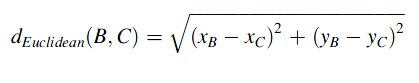
\includegraphics[scale=0.6]{images/EuclidDistance1.jpg}\\
	\end{center}
\end{figure}

The Euclidean distance is the square root of the sum of the squared differences in
the variables’ values. Suppose B and C were positioned as $(7,6)$ and $(6,5)$ respectively.
\begin{figure}[h!]
	\begin{center}
		% Requires \usepackage{graphicx}
		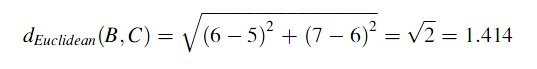
\includegraphics[scale=0.6]{images/EuclidDistance2.jpg}\\
	\end{center}
\end{figure}

This distance corresponds to the length of the line that connects objects B and C.
In this case, we only used two variables but we can easily add more under the root
sign in the formula. However, each additional variable will add a dimension to our
research problem (e.g., with ten clustering variables, we have to deal with ten
dimensions), making it impossible to represent the solution graphically.

\item  The \textbf{\textit{Squared Euclidean distance}} uses the same equation as the Euclidean distance metric, but does not take the square root. In the previous example, the squared Euclidean distance between B and C is 2.
As a result, clustering with the Squared Euclidean distance is computationally faster than clustering with the regular Euclidean distance.

\item We can compute the distance between all other pairs of objects. All
these distances are usually expressed by means of a \textit{\textbf{distance matrix}}. In this distance
matrix, the non-diagonal elements express the distances between pairs of objects
and zeros on the diagonal (the distance from each object to itself is, of course, 0). In
our example, the distance matrix is an $8 \times 8$ table with the lines and rows
representing the objects under consideration.
\begin{figure}[h!]
	\begin{center}
		% Requires \usepackage{graphicx}
		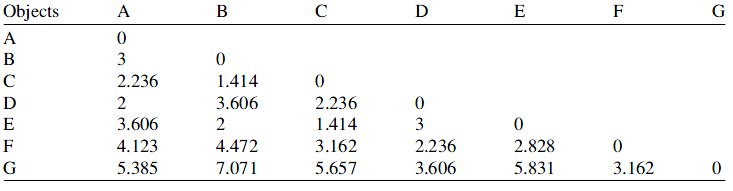
\includegraphics[scale=0.6]{images/DistanceMatrix.jpg}\\
	\end{center}
\end{figure}

\item There are also alternative distance measures: The \textbf{\textit{Manhattan distance}} or city-block distance uses the sum of the variables’ absolute differences. This is often called the Manhattan metric
as it is akin to the walking distance between two points in a city like New York’s
Manhattan district, where the distance equals the number of blocks in the directions
North-South and East-West. Using the points B and C that we used previously, the manhattan distance is computed as follows:
\begin{figure}[h!]
	\begin{center}
		% Requires \usepackage{graphicx}
		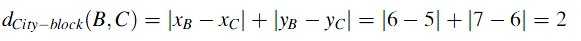
\includegraphics[scale=0.6]{images/Manhattan.jpg}\\
	\end{center}
\end{figure}


\item When working with metric (or ordinal) data, researchers frequently use
the \textbf{\textit{Chebychev distance}}, which is the maximum of the absolute difference in the
clustering variables’ values. For B and C, this result is:

\begin{figure}[h!]
	\begin{center}
		% Requires \usepackage{graphicx}
		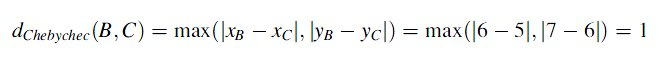
\includegraphics[scale=0.6]{images/Chebyshev.jpg}\\
	\end{center}
\end{figure}

\item There are other distance measures such as the Angular, Canberra or Mahalanobis
distance. In many situations, the \textbf{\textit{Mahalanobis
		distance}} is desirable as this measure compensates for \textbf{\textit{multi-collinearity}}
between the clustering variables. However, it is unfortunately not menu-accessible
in SPSS.
\end{itemize}
\section{Euclidean Distance}
The Euclidean distance between two points, x and y, with $k$ dimensions is calculated as:
\[ \sqrt{ \sum^{k}_{j=1} ( x_j - y_j)^2 } \]
The Euclidean distance is always greater than or equal to zero. The measurement would be zero for identical points and high for points that show little similarity.

\subsection{Example}
Compute the Euclidean Distance between the following points:
$X = \{1,5,4,3\}$ and $Y = \{2,1,8,7\}$

\begin{center}
\begin{tabular}{|c|c|c|c|}
  \hline
$x_j$	&	$y_j$	&   $x_j - y_j$	&	$(x_j - y_j)^2$	\\ \hline
1	&	2	&	-1	&	1	\\
5	&	1	&	4	&	16	\\
4	&	8	&	-4	&	16	\\
3	&	7	&	-4	&	16	\\ \hline
	&		&		&	49	\\ \hline
\end{tabular}
\end{center}
The Euclidean Distance between the two points is $\sqrt{49}$ i.e. 7.

%---------------------------------------------------------------------------%

\subsection{Squared Euclidean distance}
The most straightforward and generally accepted way of computing distances between objects in a multi-dimensional space is to compute Euclidean distances, an extension of Pythagoras's theorem.
If we had a two- or three-dimensional space this measure is the actual geometric distance between objects in the space (i.e. as if measured with a ruler).

In a univariate example, the Euclidean distance between two values is the arithmetic difference, i.e. \textbf{\textit{value1 - value2}}. In the bivariate case, the minimum distance is the hypotenuse of a triangle formed from the points, as in Pythagoras's theorem.

Although difficult to visualize, an extension of the Pythagoras's theorem will give the distance between two points in n-dimensional space. The squared Euclidean distance is used more often than the simple Euclidean distance in order to place progressively greater weight on objects that are further apart. Euclidean (and squared Euclidean) distances are usually computed from raw data, and not from transformed data, e.g. standardized data.
%----------------------------------------------------------%
\section{Standardized Euclidean distance}
The Squared Euclidean distance between two points, x and y, with $k$ dimensions is calculated as:
\[ \sum^{k}_{j=1} ( x_j - y_j)^2  \]
The Squared Euclidean distance may be preferred to the Euclidean distance as it is slightly less computational complex, without loss of any information.



Let us consider measuring the distances between between two points using
the three continuous variables pollution, depth and temperature. Let us suppose that a difference of 4.1 in terms of pollution is considered quite large and unusual, while a difference of 48 in terms of depth is large, but not particularly unusual.
What would happen if we applied the Euclidean distance formula to measure distance between two cases.
\begin{center}
\begin{tabular}{|c|c|c|}
  \hline
  % after \\: \hline or \cline{col1-col2} \cline{col3-col4} ...
Variables & case 1 & case 2 \\ \hline 
Pollution & 6.0 & 1.9 \\
Depth & 51 & 99 \\
Temp & 3.0 & 2.9 \\
  \hline
\end{tabular}
\end{center}

Here is the calculation for Euclidean Distance:
\[ d = \sqrt{(6.0 - 1.9)^2 + (51 - 99)^2 + (3.0 - 2.9)^2}   \]
 \[ d = \sqrt{16.81 + 2304 + 0.01} = \sqrt{2320.82} = 48.17 \]
\noindent The contribution of the second variable depth to this calculation is huge – one could say
that the distance is practically just the absolute difference in the depth values (equal to
$|51-99| = 48$) with only tiny additional contributions from pollution and temperature. These three variables are on
completely different scales of measurement and the larger depth values have larger differences, so they will dominate in the calculation of Euclidean distances.

\subsection*{Standardization}
\noindent The approach to take here is \textbf{standardization}, which is is necessary to balance out the contributions, and the
conventional way to do this is to transform the variables so they all have the same variance
of 1. At the same time we \textbf{\textit{center}} the variables at their means – this centering is not
necessary for calculating distance, but it makes the variables all have mean zero and thus
easier to compare. 

\noindent The transformation commonly called standardization is thus as follows:

\[\mbox{standardized value} = \frac{\mbox{observed value – mean}}{ \mbox{standard deviation}}\]
\begin{center}
\begin{tabular}{|c|c|c|c|c|c|c|}
  \hline
  % after \\: \hline or \cline{col1-col2} \cline{col3-col4} ...
Variables & Case 1 & Case 2 & Mean & Std. Dev & Case 1 (std) & Case 2 (std) \\ \hline
Pollution & 6.0 & 1.9 & 4.517	&	2.141	&	0.693	&	-1.222	\\
Depth & 51 & 99 & 74.433	&	15.615	&	-1.501	&	1.573	\\
Temp & 3.0 & 2.9 & 3.057	&	0.281	&	-0.201	&	-0.557	\\
  \hline
\end{tabular}
\end{center}

\[ d_{std} =  \sqrt{(0.693 - (- 1.222))^2 + (-1.501-1.573)^2 + (-0.201-(-0.557))^2} \]

\[ d_{std} = \sqrt{3.667 + 9.449 + 0.127} = \sqrt{13.243} = 3.639 \]

Pollution and temperature have higher contributions than before but depth still plays the
largest role in this particular example, even after standardization. But this contribution is
justified now, since it does show the biggest standardized difference between the samples. 
%--------------------------------------------------------------------------------------%
\newpage
\section{Manhattan (City Block) Distance}
The City block distance between two points, x and y, with $k$ dimensions is calculated as:
\[ \sum^{k}_{j=1} | x_j - y_j |  \]

The City block distance is always greater than or equal to zero. The measurement would be zero for identical points and high for points that show little similarity.

\subsection{Example}
Compute the Manhattan Distance between the following points: 
$X = \{1,3,4,2\}$ and $Y = \{5,2,5,2\}$


\begin{center}
\begin{tabular}{|c|c|c|c|}
  \hline
$x_j$	&	$y_j$	&   $x_j - y_j$	&	$| x_j - y_j |$	\\ \hline
1	&	5	&	-4	&	4	\\
3	&	2	&	1	&	1	\\
4	&	5	&	-1	&	1	\\
2	&	2	&	0	&	0	\\ \hline
& & & 6 \\
  \hline
\end{tabular}
\end{center}
The Manhattan Distance between the two points is 6.

%--------------------------------------------------------------------------------------%
\newpage
\subsection*{Measures for Interval Data}
The following dissimilarity measures are available for interval data:
\begin{itemize}
	
	\item Euclidean distance. The square root of the sum of the squared differences between values for the items. This is the default for interval data. {Squared Euclidean distance is the default on the classroom version of SPSS.  This is reasonable given the warning below that SPSS puts in the output.} 
	The squared Euclidean measure should be used when the CENTROID, MEDIAN, or WARD cluster method is requested.
	\item 	Squared Euclidean distance. The sum of the squared differences between the values for the items. 
	\item 	Pearson correlation. The product-moment correlation between two vectors of values. 
	\item 	Cosine. The cosine of the angle between two vectors of values. 
	\item 	Chebychev. The maximum absolute difference between the values for the items. 
	\item 	Block. The sum of the absolute differences between the values of the item. Also known as Manhattan distance. 
	\item 	Minkowski. The pth root of the sum of the absolute differences to the pth power between the values for the items. 
	\item 	Customized. The rth root of the sum of the absolute differences to the pth power between the values for the items.
\end{itemize}

\section*{Measures for Interval Data}
The following dissimilarity measures are available for interval data:
\begin{itemize}
	
	\item Euclidean distance. The square root of the sum of the squared differences between values for the items. This is the default for interval data. {Squared Euclidean distance is the default on the classroom version of SPSS.  This is reasonable given the warning below that SPSS puts in the output.} 
	The squared Euclidean measure should be used when the CENTROID, MEDIAN, or WARD cluster method is requested.
	\item 	Squared Euclidean distance. The sum of the squared differences between the values for the items. 
	\item 	Pearson correlation. The product-moment correlation between two vectors of values. 
	\item 	Cosine. The cosine of the angle between two vectors of values. 
	\item 	Chebychev. The maximum absolute difference between the values for the items. 
	\item 	Block. The sum of the absolute differences between the values of the item. Also known as Manhattan distance. 
	\item 	Minkowski. The pth root of the sum of the absolute differences to the pth power between the values for the items. 
	\item 	Customized. The rth root of the sum of the absolute differences to the pth power between the values for the items.
\end{itemize}
\section{Cluster Analysis : Proximity Matrices}

Using \textbf{\textit{nearest neighbour}} linkage, describe how the agglomeration schedule based on the following 
proximity matrix. With nearest neighbour, a case is assigned to the cluster of the case with which it has the shortest distance. Cluster are also joined on this basis.


% latex table generated in R 2.15.2 by xtable 1.7-1 package
% Tue May 14 19:17:33 2013
\begin{table}[ht]
	\centering
	\begin{tabular}{|r|rrrrrrrrrr|}
		\hline
		Case & 1 & 2 & 3 & 4 & 5 & 6 & 7 & 8 & 9 & 10 \\
		\hline
		1 & 0.00 & \textbf{4.82} & 89.39 & 85.97 & 46.26 & 71.87 & 56.42 & 23.75 & 31.57 & 11.70 \\
		2 & \textbf{4.82} & 0.00 & 94.24 & 38.96 & \textbf{5.55} & 35.07 & 74.52 & 71.27 & 61.84 & \textbf{4.84} \\
		3 & 89.39 & 94.24 & 0.00 & 57.65 & 27.27 & 25.31 & 20.89 & \textbf{2.84} & 63.50 & 89.39 \\
		4 & 85.97 & 38.96 & 57.65 & 0.00 & \textbf{22.94} & \textbf{7.13} & 70.49 & 23.09 & \textbf{12.75} & 85.97 \\
		5 & 46.26 & \textbf{5.55} & 27.27 & \textbf{22.94} & 0.00 & 39.44 & 17.43 & 79.22 & 14.47 & 46.26 \\
		6 & 71.87 & 35.07 & 25.31 & \textbf{7.13} & 39.44 & 0.00 & 27.50 & 30.65 & 13.34 & 71.87 \\
		7 & 56.42 & 74.52 & 20.89 & 70.49 & 17.43 & 27.50 & 0.00 & 91.16 & 44.92 & \textbf{6.42} \\
		8 & 23.75 & 71.27 & \textbf{2.84} & 23.09 & 79.22 & 30.65 & 91.16 & 0.00 & \textbf{3.18} & 23.75 \\
		9 & 31.57 & 61.84 & 63.50 & \textbf{12.75} & 14.47 & 13.34 & 44.92 & \textbf{3.18} & 0.00 & 31.57 \\
		10 & 11.70 & \textbf{4.84} & 89.39 & 85.97 & 46.26 & 71.87 & \textbf{6.42} & 23.75 & 31.57 & 0.00 \\
		\hline
	\end{tabular}
\end{table}


\begin{itemize}
	\item The closest pair in terms of distance (2.84) are cases 3 and 8. So this is the first linkage.
	\item The next closest pair (3.18) are 8 and 9. The next linkage joins case 9 to 3 and 8.
	\item The next closest pair (4.82) are 1 and 2. So this is the next linkage. [ So far (3,8,9) and (2,10) ] 
	\item The next closest pair (4.84) are 2 and 10. The next linkage joins case 1 to 2 and 10.
	\item The next closest pair (5.55) are 2 and 5. The next linkage joins case 5 to 1, 2 and 10. [ So far (3,8,9) and (1,2,5,10)]
	\item The next closest pair (6.42) are 7 and 10. The next linkage joins case 7 to 1, 2, 5 and 10.
	\item The next closest pair (7.13) are 4 and 6. The next linkage joins case 4 to 6. [ So far (3,8,9), (4,6) and (1,2,5,10) All cases are in clusters. This is a 3 cluster solution. ]
	\item The next closest pair (11.70) are 1 and 10. Disregard, because they are already clustered together.
	\item The next closest pair (19.44) are 4 and 9. This joins cluster (4,6) to cluster (3,8,9) [ So far (3,4,6,8,9) and (1,2,5,10). This is a 2 cluster solution.]
	\item The next closest pairing is 4 and 5. This linkage joins all cases together in one cluster.
\end{itemize}

\end{document}
